\section{Parte 3: tendencia, estacionalidad y autocorrelación}
\label{sec:parte3}

Los incisos 3.1 y 3.2 forman una descomposición clásica multiplicativa:
\[
  y_t = T_t \times S_t \times R_t,
\]
donde la tendencia $T_t$ se estima con una media móvil, el índice estacional
$S_t$ con el promedio de $y_t/T_t$ por día de la semana, y $R_t$ es lo que
queda. Todo lo genera \texttt{parte3.py}.

\subsection{Inciso 3.1: tendencia}

La media móvil centrada de 7 días es
\[
  MA_t = \frac{1}{7}\sum_{j=-3}^{3} y_{t+j},
\]
calculada sobre el calendario completo con los días cerrados en cero, como
pide el enunciado (aquí el cero es el valor correcto: el inciso 2.3 explica
por qué). Los tres primeros y los tres últimos días no tienen la ventana
completa y quedan sin valor. La figura~\ref{fig:p3_ma} la muestra sobre la
serie.

\begin{figure}[H]
  \centering
  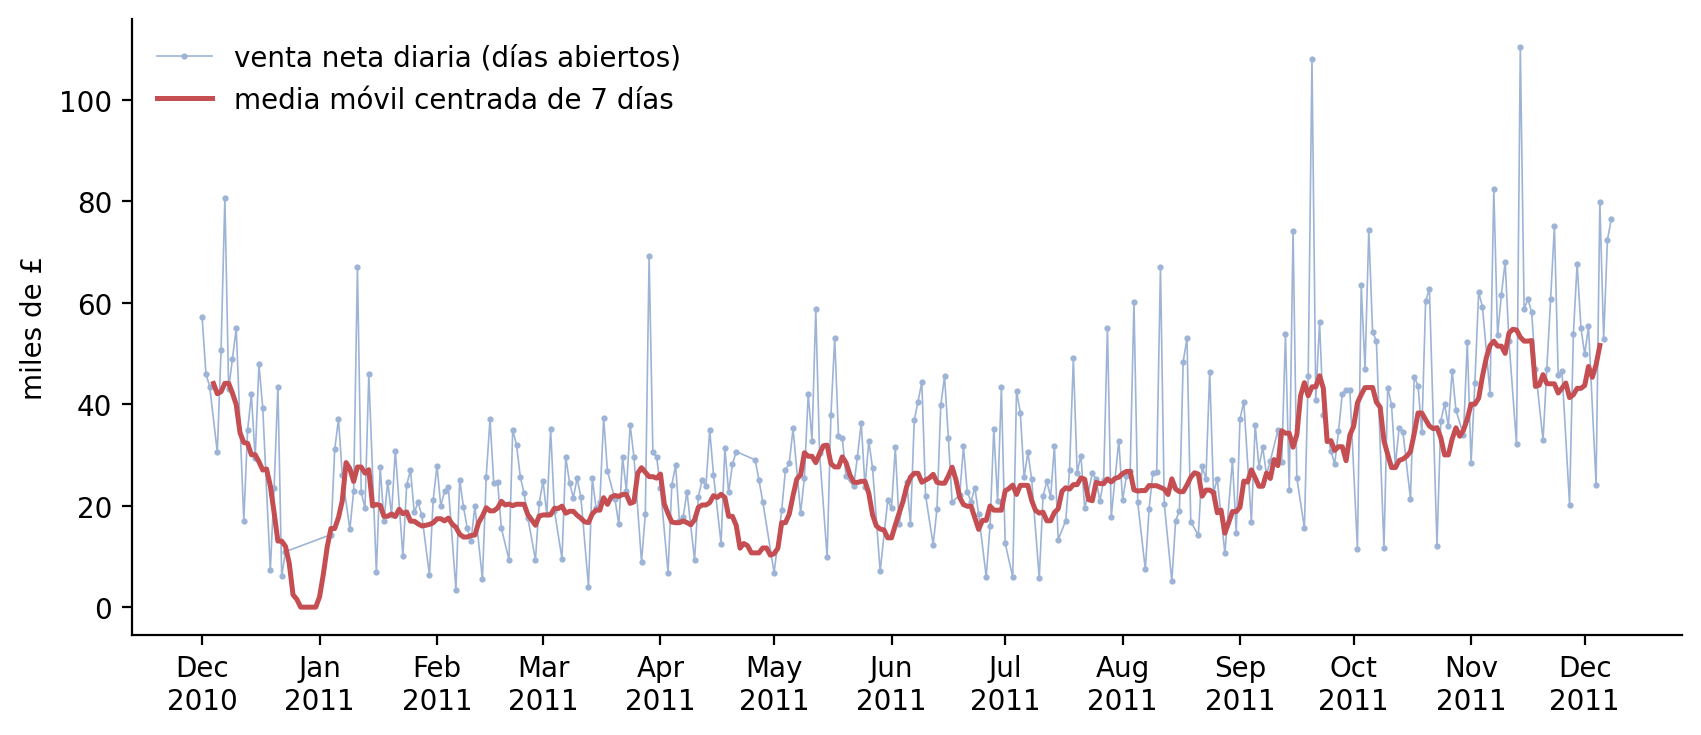
\includegraphics[width=\textwidth]{p3_media_movil.png}
  \caption{Venta neta diaria (días abiertos) y media móvil centrada de 7 días
  calculada con los días cerrados en cero.}
  \label{fig:p3_ma}
\end{figure}

\paragraph{¿Por qué 7?} Porque es el periodo del patrón semanal. Una ventana
de 7 días consecutivos contiene exactamente un lunes, un martes, \dots{} y un
sábado, así que en cada promedio entra cada día de la semana una sola vez y el
patrón semanal se cancela: lo que queda es el nivel de esa semana. Con una
ventana de 5 días la mezcla cambiaría de un día al siguiente (algunas ventanas
tendrían el sábado en cero y otras no, o dos días fuertes y ninguno débil), y
la ``tendencia'' oscilaría con periodo semanal. Con 30 días el patrón semanal
tampoco se cancela exactamente, porque 30 no es múltiplo de 7 (cada ventana
incluye dos días de la semana una vez de más), y además la ventana es tan
ancha que aplana cambios reales de nivel, como el arranque de la temporada en
septiembre o el cierre de Navidad.

\paragraph{¿Por qué centrada?} Para que $MA_t$ describa el nivel
\emph{alrededor} del día $t$, no el de los días anteriores. Una media móvil
de los últimos 7 días (de $t-6$ a $t$) mide el nivel de hace tres días y, en
una serie que sube, siempre se queda atrás. La centrada no tiene ese retraso,
y por eso sirve para descomponer y para dividir $y_t/MA_t$ en el inciso 3.2.
El costo es que usa tres días del futuro, $y_{t+1}$, $y_{t+2}$ y $y_{t+3}$:
sirve para describir la serie, no para pronosticarla. Esto vuelve a aparecer
en el inciso 5.4.

\paragraph{La tendencia.} La venta arranca en diciembre de 2010 alrededor de
\pounds40 mil diarios, se desploma a cero con el cierre de Navidad y en enero
reaparece en un nivel mucho menor. De enero a agosto queda prácticamente
plana: el promedio mensual de la media móvil se mueve entre \pounds17 y
\pounds24 mil, con altibajos de una o dos semanas pero sin dirección clara.
Desde septiembre sube con fuerza, a \pounds32 mil en septiembre, \pounds35
mil en octubre y \pounds47 mil en noviembre y diciembre, más del doble que en
la primera mitad del año. Más que una tendencia lineal es la temporada
navideña de una tienda de regalos que le vende a mayoristas: el nivel de
diciembre de 2011 se parece al de diciembre de 2010.

\subsection{Inciso 3.2: estacionalidad}

Para cada día abierto del entrenamiento se calcula el cociente $y_t/MA_t$, y
el índice estacional de cada día de la semana es el promedio de sus cocientes
(tabla~\ref{tab:p3_indices} y figura~\ref{fig:p3_indices}).

\begin{table}[H]
  \centering
  \small
  \tabla{p3_indices}
  \caption{Índices estacionales con los días abiertos del entrenamiento (1 de
  diciembre de 2010 al 30 de septiembre de 2011). ``Días'' es cuántos
  cocientes entran en cada promedio.}
  \label{tab:p3_indices}
\end{table}

\begin{figure}[H]
  \centering
  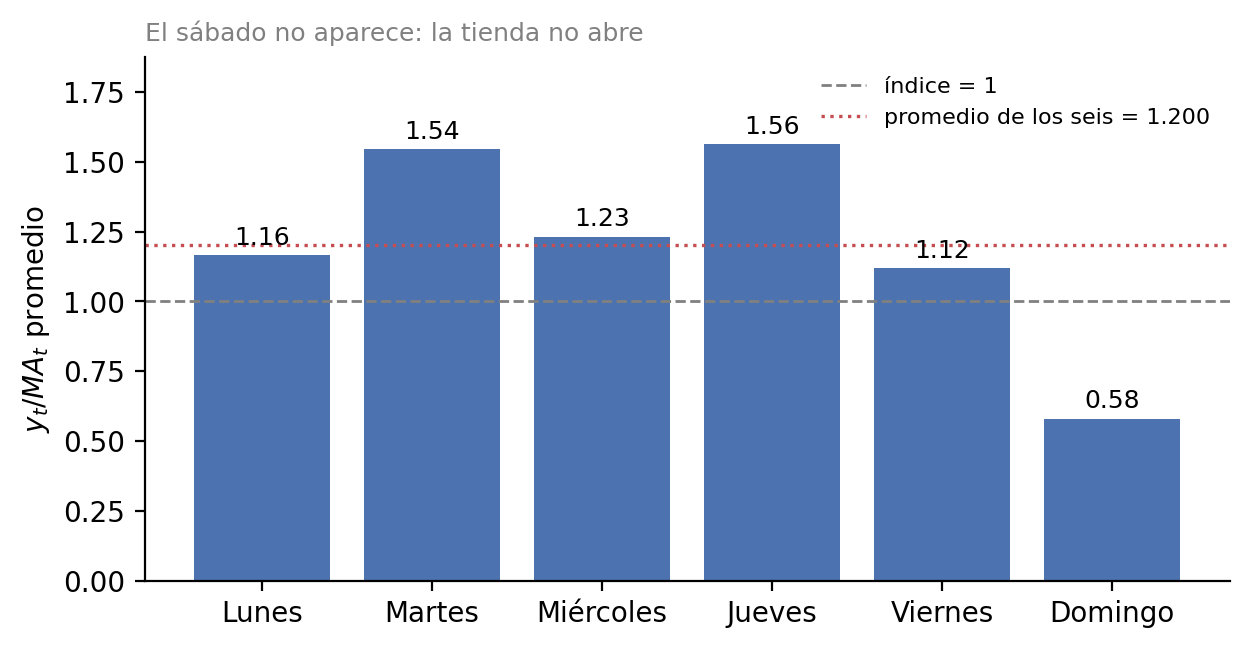
\includegraphics[width=0.75\textwidth]{p3_indices.png}
  \caption{Índice estacional por día de la semana.}
  \label{fig:p3_indices}
\end{figure}

\paragraph{¿Qué días venden más?} Martes (1.54) y jueves (1.56): esos días la
tienda vende en promedio un 55\% más que el nivel de su semana. Les siguen
miércoles (1.23), lunes (1.16) y viernes (1.12). El domingo es claramente el
día débil (0.58). Los cocientes son muy dispersos (desviaciones estándar de
0.3 a 0.5), y los mayores son martes y jueves con pedidos grandes, como el
martes 20 de septiembre, que vendió \pounds108 mil, 2.5 veces la media móvil.
Aun así, el orden no depende de esos extremos: con la mediana en lugar del
promedio, martes y jueves siguen arriba (1.44 y 1.47) y el domingo abajo
(0.53).

\paragraph{¿Por qué el promedio de los seis índices no es 1?} Porque el
séptimo día, el sábado, entra en la media móvil con un cero. Si la venta de
una semana es $V$, la media móvil vale aproximadamente $V/7$, pero esas $V$
libras se reparten entre solo seis días abiertos, que en promedio venden
$V/6$. El cociente promedio de los días abiertos es entonces
$(V/6)/(V/7) = 7/6\approx1.167$. En una descomposición clásica los siete
índices deben promediar 1, y aquí lo hacen si se cuenta el sábado con índice
cero: $(6\times1.2 + 0)/7 \approx 1.03$. El 1.200 observado queda un poco por
encima de 7/6 por dos razones: las semanas con feriado tienen todavía más
ceros en la ventana, lo que baja la media móvil y sube los cocientes de los
días vecinos (el mayor cociente del año es el martes 21 de diciembre de 2010,
justo antes del cierre de Navidad, con 3.33), y el promedio de cocientes no es
el cociente de promedios.

\subsection{Inciso 3.3: autocorrelación}

\paragraph{(a)} Se calcula $r_k$ con la función \texttt{acf} de
\texttt{series.py}, la misma de la Parte 0, sobre los 245 días abiertos del
entrenamiento puestos uno tras otro, una fila por día y sin calendario. Las
bandas son $\pm1.96/\sqrt{245}=\pm0.125$.

\begin{figure}[H]
  \centering
  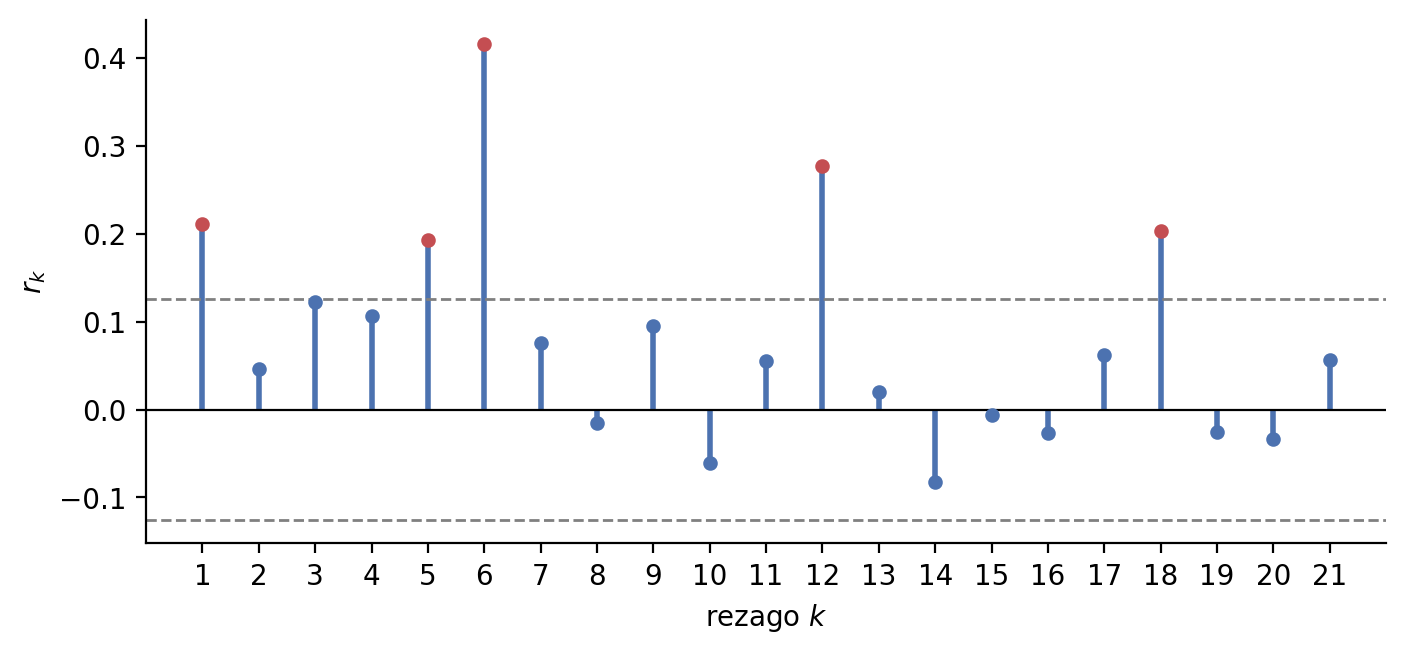
\includegraphics[width=0.85\textwidth]{p3_acf.png}
  \caption{ACF de la venta neta en los días abiertos del entrenamiento
  ($n=245$). En rojo, los rezagos fuera de las bandas.}
  \label{fig:p3_acf}
\end{figure}

\begin{table}[H]
  \centering
  \small
  \tabla{p3_acf}
  \hspace{1.5em}
  \tabla{p3_ljungbox}
  \caption{Izquierda: $r_k$ para $k=1,\dots,21$. Derecha: Ljung--Box sobre la
  serie.}
  \label{tab:p3_acf}
\end{table}

\begin{itemize}
  \item \textbf{Cinco rezagos se salen de las bandas}: 1, 5, 6, 12 y 18. Con
    21 pruebas al 5\% se esperaría uno por azar, no cinco, y menos con el
    patrón que forman.
  \item \textbf{No pasa la prueba de retardo 1} de la Tarea~2:
    $r_1=0.210>0.125$.
  \item \textbf{El pico está en $k=6$}, con $r_6=0.416$, y se repite en sus
    múltiplos: $r_{12}=0.277$ y $r_{18}=0.203$. Como la serie no tiene
    sábados, seis días abiertos hacia atrás son siete días calendario: una
    semana. De los 239 pares de días a distancia 6 en el entrenamiento, 211
    están separados exactamente por 7 días calendario; el resto están más
    separados porque entre ellos hay un feriado o el cierre de Navidad. El
    pico en 6 es el patrón semanal que encontró el inciso 3.2: un martes se
    parece al martes anterior.
  \item \textbf{Ljung--Box lo confirma}: $Q(6)=71.4$ y $Q(12)=96.9$, con
    valores-$p$ del orden de $10^{-13}$ y $10^{-15}$. La serie no es ruido
    blanco por ningún criterio.
\end{itemize}

\paragraph{(b) ¿Memoria o media no constante?} La Parte 0 enseñó a reconocer
las dos huellas. La serie tiene las dos.
\begin{itemize}
  \item Los picos en 6, 12 y 18 son la huella del proceso semanal del inciso
    0.4(b): un patrón que se repite cada semana produce autocorrelación en el
    periodo y sus múltiplos aunque no haya memoria. Es media no constante.
  \item Que casi todos los rezagos de 1 a 9 sean positivos, y que la ACF baje
    despacio, es la huella de la tendencia del inciso 0.4(a): desde septiembre
    todos los días quedan por encima de $\bar y$ y sus vecinos también. Eso
    también es media no constante.
  \item El $r_1=0.21$ puede venir de las dos cosas: de la tendencia o de
    memoria verdadera (un día de ventas altas seguido de otro igual porque los
    clientes compran en rachas). En el proceso semanal de la Parte 0 el patrón
    semanal por sí solo daba un $r_1$ ligeramente \emph{negativo}, así que el
    $r_1$ positivo no lo explica el patrón semanal.
\end{itemize}
Con solo la ACF no se puede separar cuánto es cada cosa. La receta es la del
enunciado: quitar primero la media no constante (el día de la semana, en el
inciso 4.1) y ver qué memoria le queda al residuo.
